% \subsection{Morse Code}

% \begin{frame}
%     \frametitle{Morse Code}
%         \begin{figure}
%             \caption{Morse Code By Rhey T. Snodgrass \& Victor F. Camp, 1922 - Own work based on: Intcode.png and International Morse Code.PNG, Public Domain, \url{https://commons.wikimedia.org/w/index.php?curid=3902977}}
%             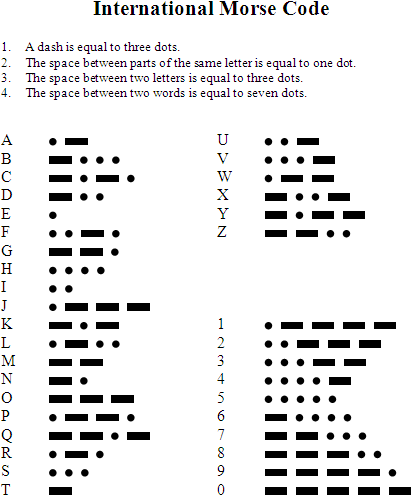
\includegraphics[scale=0.32]{../media/International_Morse_Code.png}
%         \end{figure}
%     \note{
%     }
% \end{frame}

% \begin{frame}
%     \frametitle{Morse Code - Binary Storage}
%     \begin{itemize}
%         \item Primary:
%         \begin{itemize}
%             \item dots $1'b1$
%             \item space $1'b0$
%         \end{itemize}
%         \item Secondary:
%         \begin{itemize}
%             \item dash 3 dots $3'b111$
%             \item space inside letter between dash and dots $1'b0$
%             \item space between letters $3'b000$
%             \item space between words $7'b0000000$
%         \end{itemize}
%     \end{itemize}
%     \note{
%     }
% \end{frame}

% \begin{frame}
%     \frametitle{Morse Code - Binary Tree}
%     \begin{figure}
%         \caption{Morse Code Binary Tree}
%         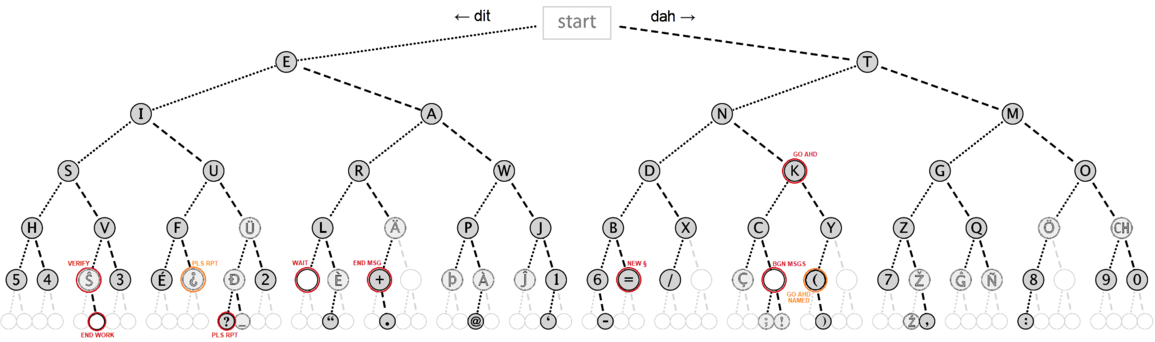
\includegraphics[scale=0.45]{../media/Morse_code_tree3.png}
%     \end{figure}
%     \note{
%     }
% \end{frame}

% \begin{frame}
%     \frametitle{Morse Code - Why not?}
%     Give up on space:
%     \begin{itemize}
%         \item dots $1'b0$
%         \item dash $1'b1$
%     \end{itemize}
%     Used today in:
%     \begin{itemize}
%         \item transmission
%         \item storage
%     \end{itemize}
% \end{frame}

\subsection{ASCII}

\begin{frame}
    \frametitle{ASCII}
    \begin{itemize}
        \item American Standard Code for Information Interchange
        \item 7-bit encoding
        \item 128 characters
        \item 33 control characters
        \item 95 printable characters
    \end{itemize}
    \note{
    }
\end{frame}


\begin{frame}
    \frametitle{ASCII Table}

    \begin{table}[h!]
        \centering
        \scalebox{0.8}{
            \begin{tabular}{|c|c|c|c|c|c|c|c|}
                \hline
                \textbf{Hex} & \textbf{Char} & \textbf{Hex} & \textbf{Char} & \textbf{Hex} & \textbf{Char} & \textbf{Hex} & \textbf{Char} \\
                \hline
                0x00 & NUL & 0x10 & DLE & 0x20 & Space & 0x30 & 0 \\
                0x01 & SOH & 0x11 & DC1 & 0x21 & ! & 0x31 & 1 \\
                0x02 & STX & 0x12 & DC2 & 0x22 & " & 0x32 & 2 \\
                0x03 & ETX & 0x13 & DC3 & 0x23 & \# & 0x33 & 3 \\
                0x04 & EOT & 0x14 & DC4 & 0x24 & \$ & 0x34 & 4 \\
                0x05 & ENQ & 0x15 & NAK & 0x25 & \% & 0x35 & 5 \\
                0x06 & ACK & 0x16 & SYN & 0x26 & \& & 0x36 & 6 \\
                0x07 & BEL & 0x17 & ETB & 0x27 & ' & 0x37 & 7 \\
                0x08 & BS  & 0x18 & CAN & 0x28 & ( & 0x38 & 8 \\
                0x09 & TAB & 0x19 & EM  & 0x29 & ) & 0x39 & 9 \\
                0x0A & LF  & 0x1A & SUB & 0x2A & * & 0x3A & : \\
                0x0B & VT  & 0x1B & ESC & 0x2B & + & 0x3B & ; \\
                0x0C & FF  & 0x1C & FS  & 0x2C & , & 0x3C & < \\
                0x0D & CR  & 0x1D & GS  & 0x2D & - & 0x3D & = \\
                0x0E & SO  & 0x1E & RS  & 0x2E & . & 0x3E & > \\
                0x0F & SI  & 0x1F & US  & 0x2F & / & 0x3F & ? \\
                \hline
            \end{tabular}
        }
        \caption{ASCII Table with Characters and Hexadecimal Values}
        \label{tab:ascii_table}
    \end{table}
\end{frame}


\begin{frame}
    \frametitle{ASCII Table}

    \begin{table}[h!]
        \centering
        \scalebox{0.8}{
            \begin{tabular}{|c|c|c|c|c|c|c|c|}
                \hline
                \textbf{Hex} & \textbf{Char} & \textbf{Hex} & \textbf{Char} & \textbf{Hex} & \textbf{Char} & \textbf{Hex} & \textbf{Char} \\
                \hline
                0x40 & @  & 0x50 & P  & 0x60 & `  & 0x70 & p \\
                0x41 & A  & 0x51 & Q  & 0x61 & a  & 0x71 & q \\
                0x42 & B  & 0x52 & R  & 0x62 & b  & 0x72 & r \\
                0x43 & C  & 0x53 & S  & 0x63 & c  & 0x73 & s \\
                0x44 & D  & 0x54 & T  & 0x64 & d  & 0x74 & t \\
                0x45 & E  & 0x55 & U  & 0x65 & e  & 0x75 & u \\
                0x46 & F  & 0x56 & V  & 0x66 & f  & 0x76 & v \\
                0x47 & G  & 0x57 & W  & 0x67 & g  & 0x77 & w \\
                0x48 & H  & 0x58 & X  & 0x68 & h  & 0x78 & x \\
                0x49 & I  & 0x59 & Y  & 0x69 & i  & 0x79 & y \\
                0x4A & J  & 0x5A & Z  & 0x6A & j  & 0x7A & z \\
                0x4B & K  & 0x5B & [  & 0x6B & k  & 0x7B & \{ \\
                0x4C & L  & 0x5C & \textbackslash  & 0x6C & l  & 0x7C & | \\
                0x4D & M  & 0x5D & ]  & 0x6D & m  & 0x7D & \} \\
                0x4E & N  & 0x5E & \textasciicircum  & 0x6E & n  & 0x7E & \textasciitilde \\
                0x4F & O  & 0x5F & \_  & 0x6F & o  & 0x7F & DEL \\
                \hline
            \end{tabular}
        }
        \caption{ASCII Table with Characters and Hexadecimal Values}
        \label{tab:ascii_table}
    \end{table}
\end{frame}




\subsection{Unicode}

\begin{frame}
    \frametitle{Unicode}
    \begin{itemize}
        \item 16-bit encoding
        \item Contains ASCII
    \end{itemize}
    \note{
    }
\end{frame}


\begin{frame}
    \frametitle{Unicode Table}

    \begin{table}[h!]
        \centering
        \scalebox{0.6}{
        \begin{tabular}{|c|c|c|c|c|c|c|c|c|c|c|c|c|c|c|c|c|}
            \hline
            \textbf{Hex} & \textbf{0} & \textbf{1} & \textbf{2} & \textbf{3} & \textbf{4} & \textbf{5} & \textbf{6} & \textbf{7} & \textbf{8} & \textbf{9} & \textbf{A} & \textbf{B} & \textbf{C} & \textbf{D} & \textbf{E} & \textbf{F} \\
            \hline
            0x0000 & NUL & SOH & STX & ETX & EOT & ENQ & ACK & BEL & BS  & TAB & LF  & VT  & FF  & CR  & SO  & SI  \\
            0x0010 & DLE & DC1 & DC2 & DC3 & DC4 & NAK & SYN & ETB & CAN & EM  & SUB & ESC & FS  & GS  & RS  & US  \\
            0x0020 & Space & ! & " & \# & \$ & \% & \& & ' & ( & ) & * & + & , & - & . & / \\
            0x0030 & 0 & 1 & 2 & 3 & 4 & 5 & 6 & 7 & 8 & 9 & : & ; & < & = & > & ? \\
            0x0040 & @ & A & B & C & D & E & F & G & H & I & J & K & L & M & N & O \\
            0x0050 & P & Q & R & S & T & U & V & W & X & Y & Z & [ & \textbackslash & ] & \textasciicircum & \_ \\
            0x0060 & ` & a & b & c & d & e & f & g & h & i & j & k & l & m & n & o \\
            0x0070 & p & q & r & s & t & u & v & w & x & y & z & \{ & | & \} & \textasciitilde & DEL \\
            \hline
        \end{tabular}
        }
        \caption{Unicode Table with Characters and Hexadecimal Values}
        \label{tab:unicode_table}
    \end{table}
    \note{
    }
\end{frame}



\begin{frame}
    \frametitle{UTF-8}
    \begin{itemize}
        \item Unicode Transformation Format
        \item 21-bit encoding
        \item Variable-width encoding (1-4 bytes)
    \end{itemize}
    \note{
    }
\end{frame}


\begin{frame}
    \frametitle{UTF-8 Encoding}
    \begin{table}[h!]
        \centering
        \scalebox{0.8}{
        \begin{tabular}{|c|c|c|}
            \hline
            \textbf{Bytes} & \textbf{Binary Format} & \textbf{Range} \\
            \hline
            1 byte  & 0xxxxxxx & U+0000 to U+007F \\
            2 bytes & 110xxxxx 10xxxxxx & U+0080 to U+07FF \\
            3 bytes & 1110xxxx 10xxxxxx 10xxxxxx & U+0800 to U+FFFF \\
            4 bytes & 11110xxx 10xxxxxx 10xxxxxx 10xxxxxx & U+10000 to U+10FFFF \\
            \hline
        \end{tabular}
        }
        \caption{UTF-8 Encoding Scheme}
        \label{tab:utf8_encoding}
    \end{table}

    \note{
    }
\end{frame}